\appendix

\begin{figure*}[htb!]
\centering
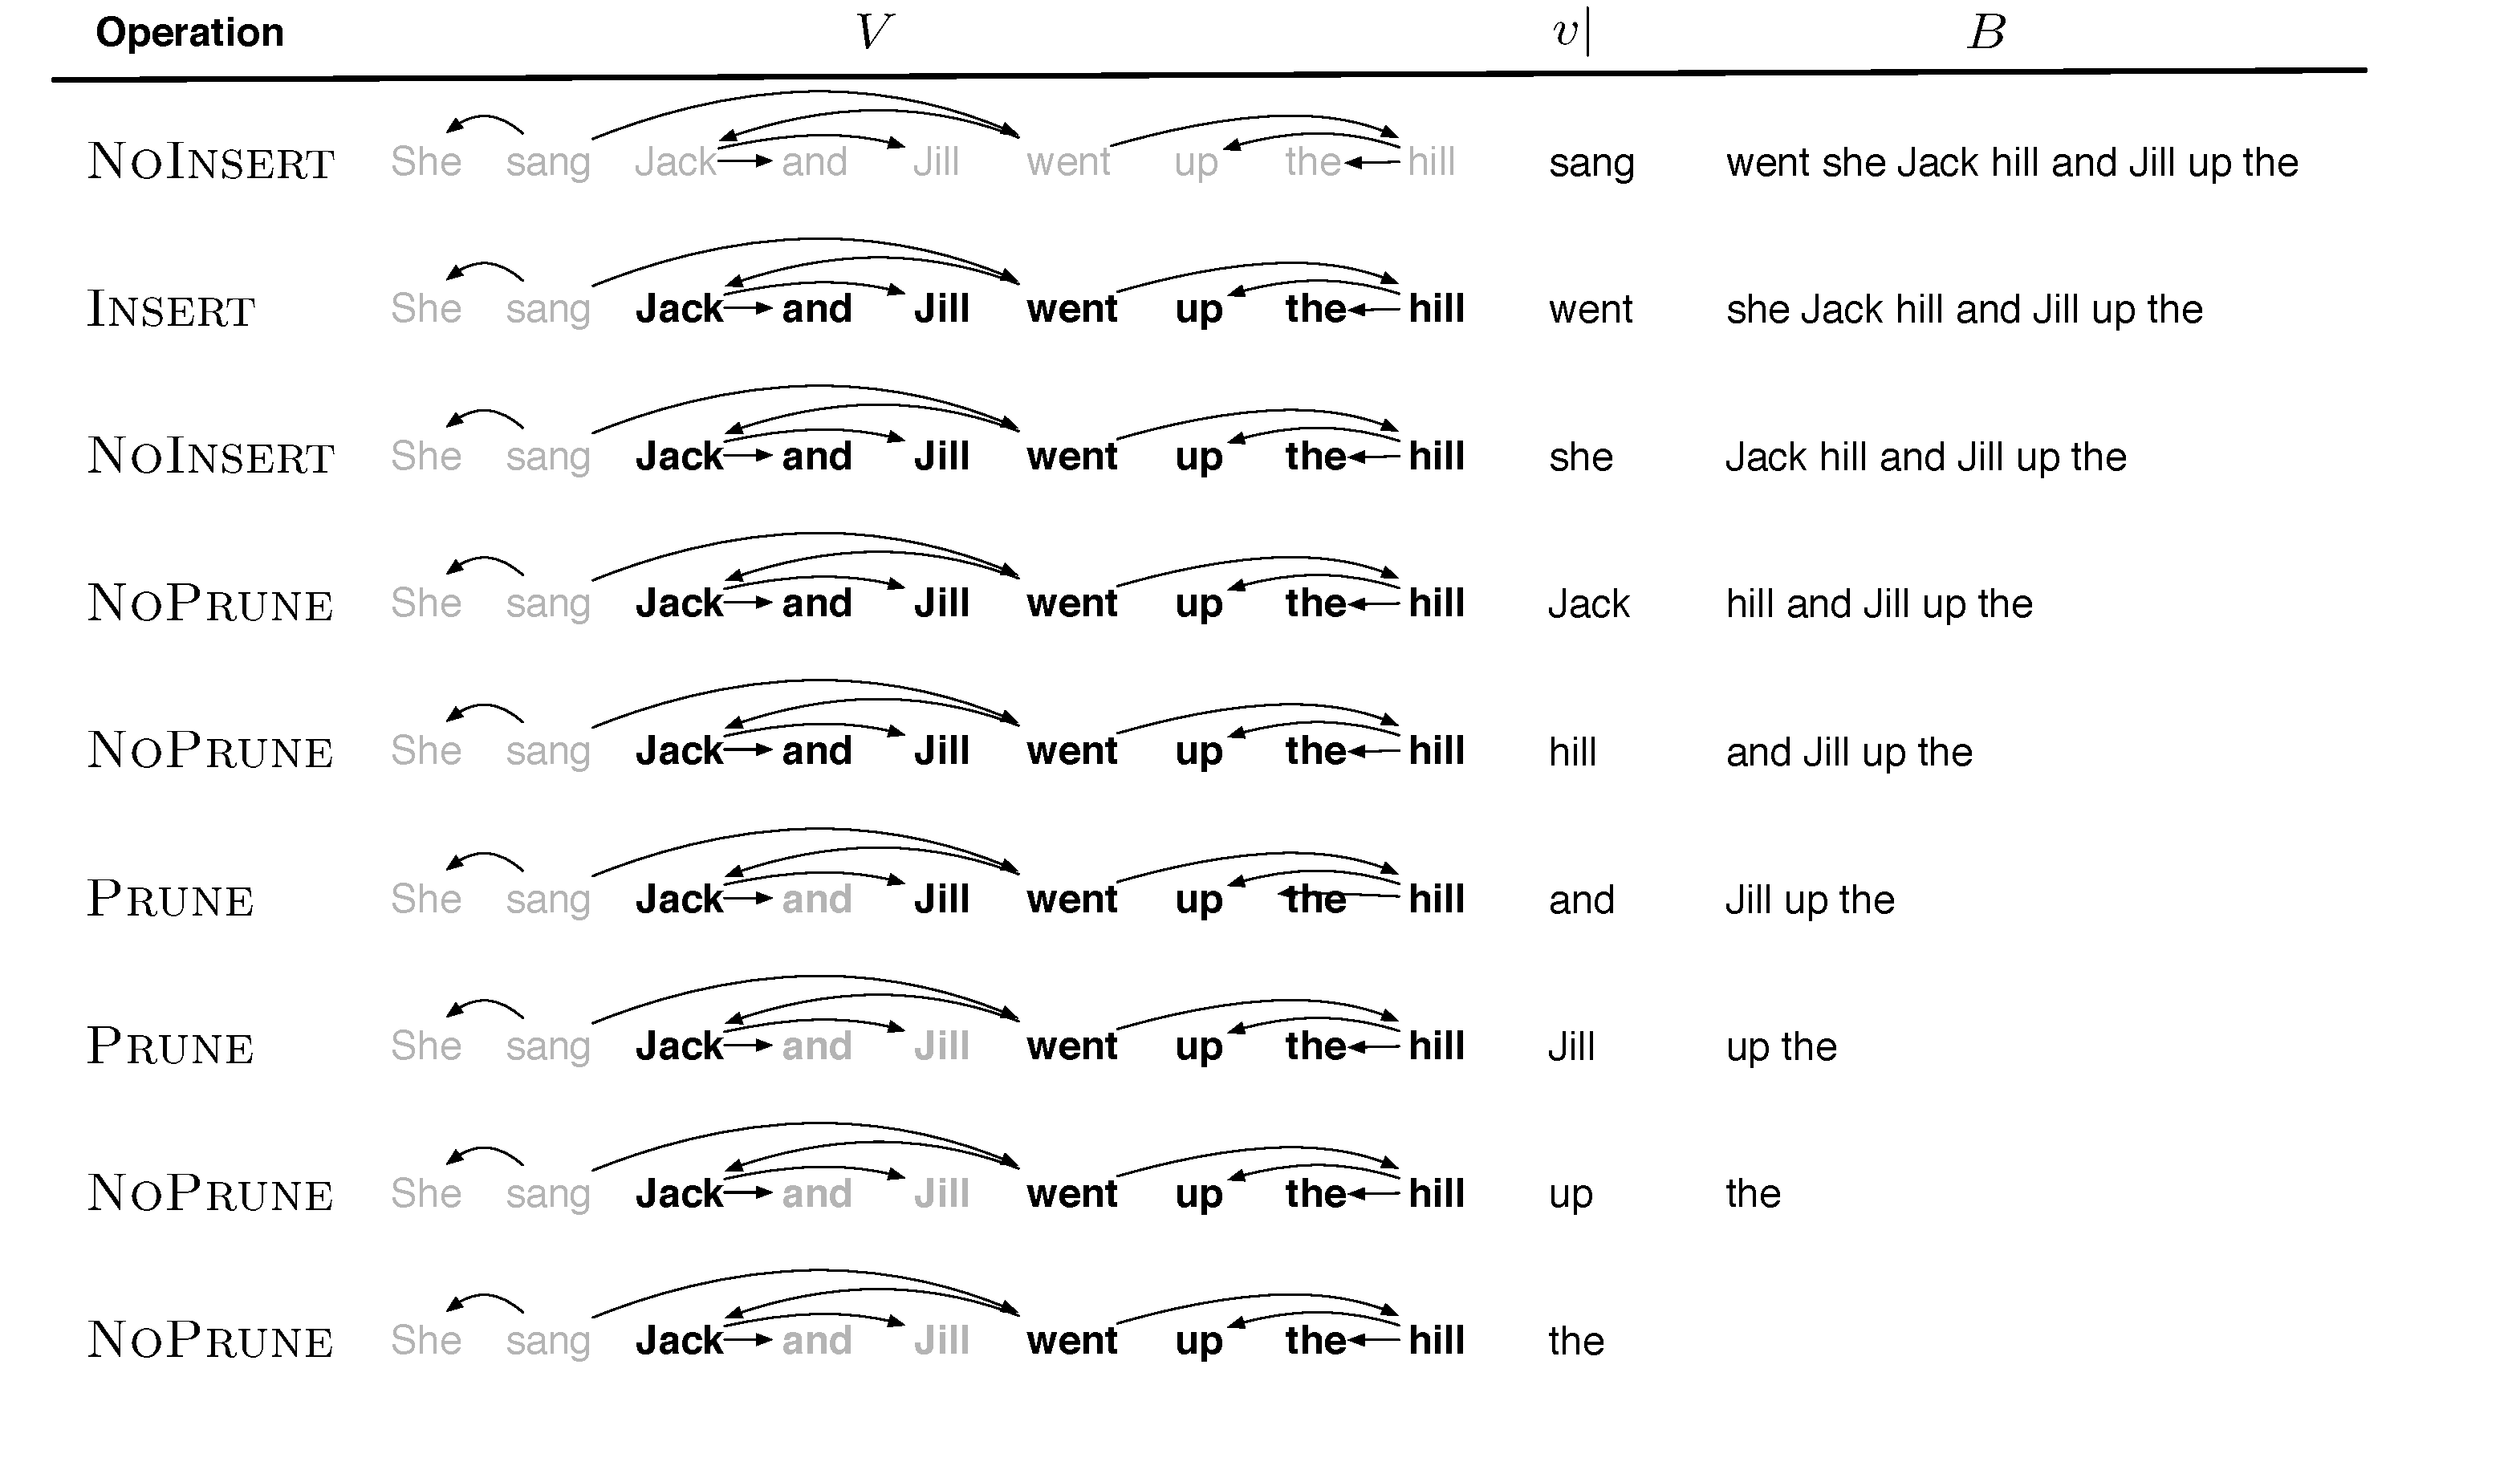
\includegraphics[width=.75\textwidth]{worked.pdf}
\caption{Nine operations of our transition-based compression return the compression: ``Jack went up the hill". At each timestep, the compression has state $(V_j, [v_j|B])$. In the diagram, the tokens in $V_j$ are shown in bold. The token $v_j$ is shown in the third column.}
\label{f:example}
\end{figure*}

\section{Appendix}

\begin{algorithm}[]
\SetKwInOut{Input}{input}
\SetAlgoLined
\Input{$s=(V,E)$, $Q \subseteq V$, $b \in \mathbb{R^+}$}
 $ C \gets Q;  F \gets V \setminus Q$; \\
 \While{ $\ell(C) < b $ and $ |F| > 0 $   }{
  $v \gets \pi(F)$; \\
  $F \gets F \setminus  \{v\}$ \\
  \If{$p(v | C) > .5$* and $\ell(C \cup \{v\}) < b$}{$C \gets C \cup \{v\}$}
 }
\KwRet{$\ell(C)$}
 \caption{Additive compression {\small(test time*)}}
\end{algorithm}\label{a:algo}

\subsection{Reimplementation of \citet{filippova2013overcoming}: additional details}

In this work, we reimplement the method of \citet{filippova2013overcoming}, who in turn implement a method partially described in \citet{filippova2008dependency}.  There are inevitable discrepancies between our implementation and the methods described in these two prior papers.  

Some discrepancies arise from differences in syntactic formalisms. To begin, prior work uses a tree transformation method which is no longer strictly compatible with UD. For instance, the tree transformation from prior work assumes PPs are headed by prepositions, which is not true in UD \cite{Schuster2016EnhancedEU}. We thus reimplement the tree transformation, using the enhanced dependencies representation from CoreNLP, which provides off-the-shelf augmented modifiers and augmented conjuncts that are very similar to the augmented edge labels from prior work. We exclude a syntactic constraint based on the \rdep{sc} relation, which is not included in UD.

Other possible discrepancies arise from differences in part-of-speech taggers. In particular, the aforementioned tree transform from prior work adds an edge between the root node and all verbs in a sentence, as a preprocessing step. This ensures that subclauses can be removed from parse trees, and then merged together to create a compression from different clauses of a sentence. However, we found that replicating this transform literally (i.e. only adding edges from the original root to all ``verbs'') made it impossible for the ILP to recreate some of the gold compressions in the dataset. (We suspect that this is because our part-of-speech tagger and the original part-of-speech tagger employed in \citet{filippova2013overcoming} sometimes return different part-of-speech tags). Our tree transform therefore adds an edge between the root node and \textit{all} tokens in a sentence. With this change, it is always possible for the ILP to output the gold compression.

We use \citet{gurobi} (v7) to solve the liner program. \citet{filippova2008dependency} report using LPsolve.\footnote{\url{http://
sourceforge.net/projects/lpsolve}}  We found that Gurobi sometimes segfaults nondeterminsitically during training. We implement checkpoints which save and restore the state of computation, allowing us to resume training when such errors occur.  We assess convergence by examining the validation F1 score on the constrained task after each pass through the training data. The F1 score increases for each of eight passes through the training data, and then decreases slightly (drops by $10^{-3}$ points). We terminate training at this point. 

Lastly, in Table 1 of their original paper, \citet{filippova2013overcoming} provide an overview of the syntactic, structural, semantic and lexical features in their model. We implement every feature explicitly described in their work, except where otherwise noted (e.g. syntactic feature not compatible with UD). However, additional features included in their model (but not explicity described in print) almost certainly affect performance. 

\subsection{Implementation of SLOR: additional details}

We use the SLOR function to measure the readability of the shortened sentences produced by each compression system. Following \cite{lau2015unsupervised}, we define the function as 

\begin{equation}
\text{SLOR}=\frac{\text{log}P_m(\xi) - \text{log}P_u(\xi)}{|\xi|}
\end{equation}

where $\xi$ is a sequence of words, $P_u(\xi)$ is the unigram probability of this sequence of words and $P_m(\xi)$ is the probability of the sequence, assigned by a language model.  $|\xi|$ is the length (in tokens) of the sentence.

We use a 3-gram language model trained on the \citet{filippova2013overcoming} corpus. We implement with KenLM \cite{Heafield-kenlm}.

\bibliography{abe}
\bibliographystyle{acl_natbib}